%; whizzy chapter
% -initex iniptex -latex platex -format platex -bibtex jbibtex -fmt fmt
% 以上 whizzytex を使用する場合の設定。

%     Kansai Debian Meeting resources
%     Copyright (C) 2007 Takaya Yamashita
%     Thank you for Tokyo Debian Meeting resources

%     This program is free software; you can redistribute it and/or modify
%     it under the terms of the GNU General Public License as published by
%     the Free Software Foundation; either version 2 of the License, or
%     (at your option) any later version.

%     This program is distributed in the hope that it will be useful,
%     but WITHOUT ANY WARRANTY; without even the implied warranty of
%     MERCHANTABILITY or FITNESS FOR A PARTICULAR PURPOSE.  See the
%     GNU General Public License for more details.

%     You should have received a copy of the GNU General Public License
%     along with this program; if not, write to the Free Software
%     Foundation, Inc., 51 Franklin St, Fifth Floor, Boston, MA  02110-1301 USA

%  preview (shell-command (concat "evince " (replace-regexp-in-string "tex$" "pdf"(buffer-file-name)) "&"))
% 画像ファイルを処理するためにはebbを利用してboundingboxを作成。
%(shell-command "cd image200708; ebb *.png")

%%ここからヘッダ開始。

\documentclass[mingoth,a4paper]{jsarticle}
\usepackage{kansaimonthlyreport}
\usepackage[dvips]{xy}


% 日付を定義する、毎月変わります。
\newcommand{\debmtgyear}{2012}
\newcommand{\debmtgdate}{27}
\newcommand{\debmtgmonth}{5}
\newcommand{\debmtgnumber}{59}

\begin{document}

\begin{titlepage}

% 毎月変更する部分、本文の末尾も修正することをわすれずに

 第\debmtgnumber{}回 関西 Debian 勉強会資料

\vspace{2cm}

\begin{center}
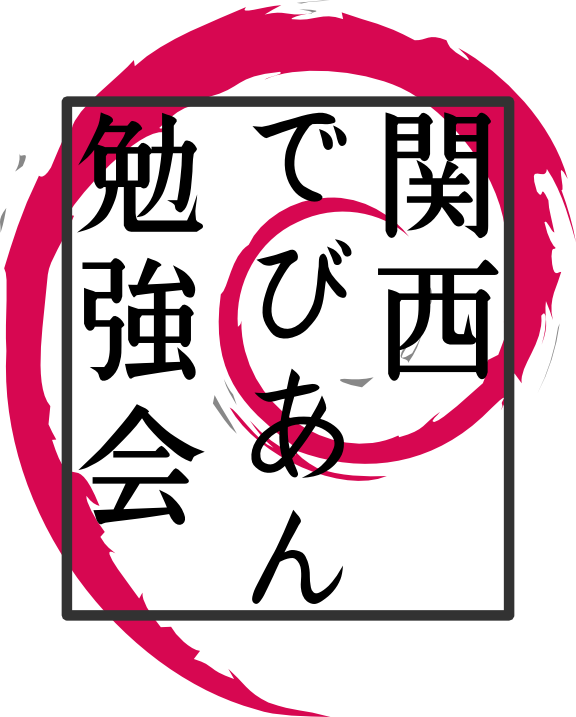
\includegraphics{image200802/kansaidebianlogo.png}
\end{center}

\begin{flushright}
\hfill{}関西 Debian 勉強会担当者 佐々木・倉敷・のがた・かわだ \\
\hfill{}\debmtgyear{}年\debmtgmonth{}月\debmtgdate{}日
\end{flushright}

\thispagestyle{empty}
\end{titlepage}

\dancersection{Introduction}{Debian JP}

 関西Debian勉強会はDebian GNU/Linuxのさまざまなトピック
 (新しいパッケージ、Debian特有の機能の仕組、Debian界隈で起こった出来事、
 などなど)について話し合う会です。

 目的として次の三つを考えています。
 \begin{itemize}
  \item MLや掲示板ではなく、直接顔を合わせる事での情報交換の促進
  \item 定期的に集まれる場所
  \item 資料の作成
 \end{itemize}

 それでは、楽しい一時をお楽しみ下さい。

\newpage

\begin{minipage}[b]{0.2\hsize}
 {\rotatebox{90}{\fontsize{80}{80}
{\gt 関西 Debian 勉強会}}}
\end{minipage}
\begin{minipage}[b]{0.8\hsize}
\hrule
\vspace{2mm}
\hrule
\setcounter{tocdepth}{1}
\tableofcontents
\vspace{2mm}
\hrule
\end{minipage}

\dancersection{最近のDebian関係のイベント報告}{Debian JP}

\subsection{第 58 回関西 Debian 勉強会}
58 回目の関西 Debian 勉強会は 4 月 22 日に開催されました。

著作権入門と konoha のパッケージ作成、そして月刊企画の Debian Policy は第2章の
Debian アーカイブについてのお話でした。

パッケージ作成のお話はもう月刊企画になりつつありよい感じです。
konoha はアップストリームの動向待ちになり Wheezy には間に合わないようですが、
整理されて Debian にパッケージが入る日が早く来るといいですね。


\subsection{第 88 回東京エリア Debian 勉強会}
88 回目の東京エリア Debian 勉強会は 5 月 19 日に開催されました。

Python と coffeescript というスクリプト二本立てのお話しでした。

Debian で Python の環境を整えようと思われる方には参考になると思います。

coffeescript はまだ Wheezy に入っていないようですが、Debian での JavaScript 環境
も整いつつあるようですね。

\clearpage

\dancersection{事前課題}{Debian JP}

今回は以下の課題を出題しました.
\begin{screen}
  \begin{enumerate}
  \item ITPをしたことがない方は、ITPしたいパッケージを探してみて概要を紹介してください。\\
    (\url{http://www.debian.org/devel/wnpp/}から探すのもよいでしょう。)\\
     ITPをしたことがある方は、最初のITPパッケージの概要とITPをするきっかけなどを語ってください。

   \item Essential なパッケージをひとつ挙げてパッケージのコントロールフィールドを確認し
     \begin{description}
     \item アーカイブエリア
     \item アーカイブセクション
     \item パッケージ名
     \item バージョン
     \item メンテナ
     \end{description}
     をおしえてください。そのメンテナが個人かグループかも判定して下さい。
  \end{enumerate}
\end{screen}

参加者の皆さんの解答は以下の通りです.

\begin{prework}{ 佐々木洋平 }
  \begin{enumerate}
  \item rttool、だった気がする。
  \item 
    \begin{description}
    \item [アーカイブ] main
    \item [アーカイブセクション] libs
    \item [パッケージ名] libc-bin
    \item [バージョン] 2.13-32
    \item [メンテナ] GNU Libc Maintainers $<$debian-glibc@lists.debian.org$>$
      \begin{description}
      \item Team ですね。
      \end{description}
    \end{description}
  \end{enumerate}
\end{prework}

\begin{prework}{ 川江 }
  \begin{enumerate}
  \item
    \begin{description}
    \item [PPP] ポイント to ポイントでパソコン同士を繋ぐパッケージ
    \end{description}
  \item dpkg main dpkg 1.16.3 Dpkg Developers
  \end{enumerate}
\end{prework}

\begin{prework}{ のがたじゅん }
  \begin{enumerate}
  \item ITPはしたことないです。してみたいなと思ってるソフトを挙げてみた(てか、その後の言葉が予想出来るだけに無理はしてないはず)
    \begin{description}
    \item [luppp] Abelton Liveに似たオーディオ・ループ・シーケンサー。
      \begin{description}
      \item \url{https://github.com/harryhaaren/Luppp/}
      \item ライセンスはGPL3。
      \item Linuxでライブ演奏に使えるシーケンサーがないから注目してるけど、超アルファすぎてビルドすらままならず。makeじゃなくてwafとか使ってたりいろいろ調べなきゃなーと思って放置。
      \end{description}
    \item [cromfs] ユーザー空間で利用できる圧縮ROMファイルシステム
      \begin{description}
      \item \url{http://bisqwit.iki.fi/source/cromfs.html}
      \item ライセンスはGPL3
      \item すげー昔、regretとか作ってた時、おっそろしく圧縮に時間かかるのに展開が早くてライブCDとかに良さそうだなーと思った圧縮ROMファイルシステム。忘れてたので思い出した。
      \end{description}
    \item [AzMiniPainter] ドット線描画用の簡易ペイントソフト
      \begin{description}
      \item \url{http://hp.vector.co.jp/authors/VA033749/linux/index.html}
      \item ライセンスはGPL3/ライブラリはLGPL3
      \item AzPainterの人が作ってるからビルドしてみたいなーと思いつつ手を出していないから。
      \end{description}
    \end{description}
  \item build-essentialにある/usr/share/build-essential/essential-packages-listを見ました。\\
    その中からbase-filesを見ました。
    \begin{description}
    \item [アーカイブエリア] main
    \item [アーカイブセクション] admin
    \item [パッケージ名] base-files
    \item [バージョン] 3.9.1
    \item [メンテナ] Santiago Vila $<$sanvila@debian.org$>$ さん
    \end{description}
    個人だと思います。
  \end{enumerate}
\end{prework}

\begin{prework}{ かわだてつたろう }
  \begin{enumerate}
  \item
    \begin{description}
    \item [stl-manual] C++-STL documentation in HTML
      \begin{description}
      \item SGI の STL プログラマーズガイド
      \item (ITA され RFS も出されていますが止まっているようです。)
      \end{description}
    \end{description}
  \item 
    \begin{description}
    \item [アーカイブエリア] main
    \item [アーカイブセクション] utis 
    \item [パッケージ名] grep
    \item [バージョン] 2.12-2
    \item [メンテナ] Anibal Monsalve Salazar $<$anibal@debian.org$>$
    \end{description}
    メンテナは個人です。\\
    アーカイブエリアはコントロールフィールドに記載されていませんでしたが、Essential なパッケージなので main 以外にないでしょう。
  \end{enumerate}
\end{prework}

\begin{prework}{ 山城の国の住人 久保博 }
  \begin{enumerate}
  \item ITPしたことがありません。するとすれば、次のソフトかな。でも、似たような etherwake や wakeonlan というパッケージがあるので、 ITP する意義が薄い気がしています。
    \begin{description}
    \item [wakeoverlan] と名づけている、自作の C プログラム。 Wake On LAN パケットを指定した IP アドレスへ向けて飛ばす。
    \end{description}
  \item aptitude ?Essential で出した一覧から sed を選びました。\\
    squeeze 環境で、
    \begin{description}
    \item [アーカイブエリア] main
    \item [アーカイブセクション] utils
    \item [パッケージ名] sed
    \item [バージョン] 4.1.5-6
    \item [メンテナ] Clint Adams $<$schizo@debian.org$>$
    \end{description}
    でした。BTS でのやりとりの様子を見るに、メンテナは実在の人だと思います。
  \end{enumerate}
\end{prework}

\begin{prework}{ lurdan }
  \begin{enumerate}
  \item
    \begin{description}
    \item [yaskkserv] 当時、アーカイブにある skkserv はほとんどメンテされていない昔の残骸ばかりでした。自分で使う上で apt-get で入って欲しかったので、自分でつっこむことにしました。
    \end{description}
  \item 何かと話題の sysvinit
    \begin{description}
    \item [アーカイブエリア] main
    \item [アーカイブセクション] admin
    \item [パッケージ名] sysvinit
    \item [バージョン] 2.88dsf-22.1
    \item [メンテナ] Debian sysvinit maintainers (グループ)
    \end{description}
  \end{enumerate}
\end{prework}

\begin{prework}{ yyatsuo }
  \begin{enumerate}
  \item
    \begin{description}
    \item [lpc21isp] ARMマイコン書き込み用ISPツール
    \end{description}
  \item 
    \begin{description}
    \item [アーカイブエリア] main
    \item [アーカイブセクション] utils
    \item [パッケージ名] coreutils
    \item [バージョン] 8.13-3.2
    \item [メンテナ]  Michael Stone 
    \end{description}
  \end{enumerate}
\end{prework}

\begin{prework}{ 西山和広 }
  \begin{enumerate}
  \item ITP はしたことがありません。\\
    気になっているものとしては

    \#638838 - ITP: cocot -- Wraps and converts charset encoding of program input/output. - Debian Bug report logs\\
    \url{http://bugs.debian.org/cgi-bin/bugreport.cgi?bug=638838}\\
    があります。\\
    script コマンドのように端末とプログラムの間に入って、エンコーディング変換をしてくれるプログラムです。\\
    EUC-JP の環境が混在していたときには非常に便利でした。\\
    今でもルーターに telnet でつなぐときに Shift\_JIS との変換に使うなど便利に使っています。\\
    \\
    もう一つ気になっているものとしては ccollect があります。\\
    \url{http://www.nico.schottelius.org/software/ccollect/}\\
    rsync の --link-dest を使って pdumpfs のような変化のなかったファイルはハードリンクにするというバックアップをとれるプログラムです。\\
    シェルスクリプトによる実装で依存が少ないのも魅力です。
  \item Essential なパッケージは aptitude search '\textasciitilde{}E' または aptitude search '?essential' で探せました。 squeeze では 25 個のパッケージが Essential になっていました。\\
    その中から最初に思いついていた apt を選びました。
    \begin{description}
    \item [アーカイブエリア] main
    \item [アーカイブセクション] admin
    \item [パッケージ名] apt
    \item [バージョン] 0.8.10.3+squeeze1
    \item [メンテナ] APT Development Team $<$deity@lists.debian.org$>$
    \end{description}
    でグループメンテナでした。\\

    全体としては
    \begin{description}
    \item [アーカイブエリア] すべて main
    \item [アーカイブセクション] admin: 10, perl: 2, shells: 2, utils: 12
    \end{description}
    となっていました。
  \end{enumerate}
\end{prework}

\begin{prework}{ よだ たくや }
  \begin{enumerate}
  \item
    \begin{description}
    \item [ITP経験] なし
    \item [ITPしたいパッケージ] 思いつきませんでした。
    \end{description}
  \item 
    \begin{description}
    \item [アーカイブエリア] main
    \item [アーカイブセクション] utils
    \item [パッケージ名] tar
    \item [バージョン] 1.26-4
    \item [メンテナ] Bdale Garbee
    \end{description}
  \end{enumerate}
\end{prework}

\begin{prework}{ 甲斐正三 }
  事前課題の回答は以下のとおりです。
  \begin{enumerate}
  \item 
    'ITP'はできませんが、'jfbterm'には関心がありますので、調べた結果を報告します。(Squeeze上'aptitude show'による)\\
    フルネームは'J Framebuffer Terminal/Multilingual Extension'と言い、フレームバッファ上でCJKマルチリンガルテキストを表示するソフトウエアである。
    \item essential(必須)なソフトウエアとして'dpkg'を揚げました。
      \begin{description}
      \item [アーカイブエリア] main
      \item [アーカイブセクション] admin
      \item [パッケージ名] dpkg
      \item [バージョン] 1.16.3
      \item [メンテナー] Dpkg Developers(グループのようです)
      \end{description}
  \end{enumerate}
  以上よろしくお願いします。
\end{prework}

\begin{prework}{ kozo2 }
  \begin{enumerate}
  \item ITPの課題:
    \begin{description}
    \item [Cytoscape] というネットワーク可視化ソフト

      \#465331を見る限りではITPからRFPにステータスが変わったようだった。Javaアプリなので大変そうではあるが興味がある。
    \end{description}
  \item コントロールフィールド確認の課題:
    \begin{description}
    \item [アーカイブエリア] パッケージディレクトリにない
    \item [アーカイブセクション] パッケージディレクトリにない
    \item [パッケージ名]: emacs-snapshot
    \item [バージョン] 2:20120521-1
    \item [メンテナ] Julien Danjou(個人)
    \end{description}
  \end{enumerate}
\end{prework}

\begin{prework}{ よしだともひろ }
  \begin{enumerate}
  \item 3月31日にsdic-inline-elでITPデビューしました。
    \begin{description}
    \item [sdic-inline-el] はポイント下の単語の意味をミニバッファに表示するEmacs Lispです。
    \end{description}
    普段からsdic-inlineを使っていて、まだDebianパッケージになっていなかったので思い切ってITPしてみました。
  \item aptitude search \textasciitilde{}E で essentialなパッケージを探しsedのcontrolファイルを見ました。
    \begin{description}
    \item [アーカイブエリア] main
    \item [アーカイブセクション] utils
    \item [パッケージ名] sed
    \item [バージョン] 3.9.1
    \item [メンテナ] Clint Adams(個人)
    \end{description}
  \end{enumerate}
\end{prework}

\clearpage

\dancersection{ITP から始めるパッケージメンテナへの道}{よしだ ともひろ}
\subsection{はじめに}
とある便利なソフトウェアを見つけて、それがまだDebianパッケージになっていなかった
とき、RFP(Request For Package:パッケージ化の要求)をしてもよいのですが、自分でパッ
ケージ化してDebianの一部として提供することもできます。そこで、ITP(Intent To Package:
パッケージ化の宣言)〜アップロードまでの流れをまとめてみました。

\subsection{まずはITP}
\subsubsection{ITPの前に必要なこと}
\subsubsubsection{既にパッケージ化されていないか?}
\url{http://www.debian.org/distrib/packages}で探してみたり、aptitude searchや
apt-cache searchで確認してみましょう。

\subsubsubsection{既にITPされていないか?}
他の誰かが同じようにパッケージ化しようと思って、ITPしているかもしれません。

\url{http://www.debian.org/devel/wnpp/being\_packaged}をチェックしてみましょう。

\subsubsubsection{既にRFPされていないか?}
他の誰かが、パッケージ化して欲しいと思って、RFPしているかもしれません。
RFPされている場合は、ITPすることでパッケージ化の宣言を行います。

\url{http://www.debian.org/devel/wnpp/requested}をチェックしてみましょう。

\subsection{ITPの仕方}
パッケージをITPするのはreportbug(apt-get|aptitude install reportbug)で行う方法が
\url{http://www.debian.org/devel/wnpp/}で紹介されています。また、電子メールでも
行うことができます。ここでは、電子メールでITPを行う方法の一つ、Mewを使う方法を
紹介します。

まず、debian-elパッケージをインストールします。

\begin{commandline}
   $ sudo aptitude install debian-el
\end{commandline}
%$ for emacs font-lock
 
   次に~/.emacsに以下を追加します。

\begin{commandline}
(autoload 'mew "mew" nil t)
(autoload 'mew-send "mew" nil t)

(if (boundp 'read-mail-command)
	(setq read-mail-command 'mew))
(autoload 'mew-user-agent-compose "mew" nil t)
(if (boundp 'mail-user-agent)
	(setq mail-user-agent 'mew-user-agent))
(if (fboundp 'define-mail-user-agent)
	(define-mail-user-agent
		'mew-user-agent
		'mew-user-agent-compose
		'mew-draft-send-message
		'mew-draft-kill
		'mew-send-hook))
\end{commandline}

こうしておいてemacsを起動し、M-x debian-bug RETとします。
ミニバッファに

\begin{commandline}
Report a bug for a [P]ackage or [F]ile: (default P) 
\end{commandline}

と表示されるので"P"を入力します。

パッケージ名を聞いてきますのでwnppと入力します。wnppというのはWork-Needing and
Prospective Packages(作業が望まれるパッケージ)という擬似パッケージのことで、ITP
やRFPを行うときに使用する他、RFH(Request For Help:助力の要求)、RFA(Request For
Adoption:養子引き取りの要求)、O(Orphan:みなしご)、ITA(Intent To Adopt:養子引き
取りの表明)にも使います。

次にActionを聞かれます。TABを押すと候補が表示されますのでITPとします。

あとは、パッケージ名、パッケージの簡単な説明を入力します。debian-develへCCするか?
も聞かれますので"y"と入力するとメールの雛形が表示されますので、残りのVersion、
Upstream Author、URL or Web page、Licenseを入力してメールを送信します。

\subsection{GnuPGキーサイン}
Debian公式パッケージにするにはdscファイルとchangesファイルに署名が必要です。
GnuPG(GPG)で署名しますが、信頼された鍵でないと意味がないのでキーサインパーティな
どでDebian開発者の方とキーサインをしておきましょう。GPG公開鍵は後に説明する
mentors.debian.netを使う時にも必要ですので、まだ、作成していない方は作っておくこ
とをおすすめします。

6月23日(土)の大統一Debian勉強会でもキーサインパーティが予定されていますので、
是非参加しましょう。

\subsection{パッケージ作成}
パッケージの作成方法は過去のDebian勉強会などでも何度か紹介されていますので、
ここでは詳細は割愛し注意する箇所のみとします。

\subsubsection{lintian cleanにする}
lintianはDebianパッケージを精査し、バグやポリシー違反を報告します。アップロードす
る前に、必ずそのパッケージに対してlintianを実行してください。lintianを実行する際
はオプションの -v を付けてchangesファイルを指定します。lintianが出力する情報がわ
かりにくければ -i オプションを追加しましょう。出力される情報に "E:" や "W:"がなく
なるように修正し、lintian cleanにしましょう。

\subsubsection{パッケージに署名する}
お試しでパッケージを作ったりする場合はパッケージへの署名を省略しますが、公式パッ
ケージにするにはちゃんと署名することが必要です。debuildやdpkg-buildpackageで-us -uc
オプションをつけずにパッケージ作成すると、dscファイルとchangesファイルにGnuPGで署
名すためのパスフレーズを聞いてきますので入力すればOKです。

\subsection{mentors.debian.netへ登録}
\subsubsection{mentors.debian.netとは}
Debianへのパッケージアップロード権限はDebian開発者のみが持っているのですが、Debian
開発者でない人もアップーロードできる仕組みがあります。Debian開発者の方にスポンサー
になっていただいて、助言をいただきながら修正していく場、といった感じです。

\subsubsection{サインアップ}
\url{http://mentors.debian.net/}に"Sign me up"という
\url{http://mentors.debian.net/register/register}へのリンクがありますのでクリック
します。

Full name, E-mail, Password, Confirm passwordを入力し、Account typeはMaintainerを
選択してSubmitを押下します。入力したE-mail Addressへ確認のメールが飛んできますの
で、記載されたURLへアクセスしてActivateするとアカウントが使用可能になります。

ログインして、My accountページのChange GPG keyでGPGキーを登録できますのでアスキー
形式でエクスポートした公開鍵のファイルを選択して登録しておきます。

\subsubsection{アップロード}
mentors.debian.netにアップロードする方法は、duploadやdputなどのツールで行えます。
今回はdputで行う方法をご紹介します。

\begin{enumerate}
\item 準備

\textasciitilde/.dput.cfを作ります。内容は\url{http://mentors.debian.net/intro-maintainers}を
参考にしました。httpとftpの設定が記載されているのですが、httpの設定としました。
こんな感じです。

\begin{commandline}
[mentors]
fqdn = mentors.debian.net
incoming = /upload
method = http
allow_unsigned_uploads = 0
progress_indicator = 2
# Allow uploads for UNRELEASED packages
allowed_distributions = .*
\end{commandline}

\item さあ、アップロード

いよいよアップロードです。dput mentors changesファイル で行います。ここまでのパッ
ケージ作成で問題がなければmentors.debian.netへのアップロードは成功するはずです。

しばらくするとmentors.debian.netからメールが飛んできます。メールの内容は「スポン
サーが必要ならスポンサーを探してるにしろ」とか、「RFS(request for sponsorship)で
スポンサーを募集できるよ」というような内容ですので従います。
\end{enumerate}

\subsection{スポンサーを探す}
無事 mentors.debian.net へアップロードできたら debian-mentors@lists.debian.org や
debian-devel@debian.or.jp にRFS(request for sponsorship)を投げて、スポンサーになっ
てくれる方を探しましょう。

\subsection{おわりに}
今回、はじめてITPして、mentors.debian.netにアップロードしてみました。色々調べたり
しながらでしたので時間はかかりましたが、それほど難しくはないと思います。Debianパッ
ケージになっていないソフトウェアを見つけたら是非ITPしましょう!

\clearpage

%% -*-tex-*-
%%
%% Copyright (C) 2012 Hiroshi Kubo  all rights reserved.
%% 本資料の著作権は、著者である久保博 <h-kubo@geisya.or.jp> にあります。
%% Debian Policy とその日本語訳の引用があります。
%%
%% This document material is licensed under the GNU General Public License version 2.0.
%% This document is originally in the form of LaTeX source code. This shall be referenced as the ``Corresponding Source''
%% Any compiled forms including DVI, Postscript, and PDF from the original source code shall be reference as the ``Object code''.
%%
%%
%% Debian Policy は、
%%  1996, 1997, 1998, Ian Jackson and Christian Schwarz
%%   1999, Software in the Public Interest, Inc.
%%   1999-2012, many other Debian contributors
%% による著作です。
%% 取得元は : git://git.debian.org/git/dbnpolicy/policy.git です。
%%
%% Debian Policy 日本語訳は八田真行氏 mhatta@debian.or.jp 、かねこ氏 skanek@a2.mbn.or.jp、 森本氏 odin@sleipnir.dice.cache.waseda.ac.jp 
%% による著作です。
%% 取得元は : https://svn.debian.or.jp/repos/www/trunk/src/community/devel/debian-policy-ja/policy.ja.sgml  です。
\dancersection{月刊 Debian Policy 第4回 「バイナリパッケージ」}{山城国の住人 久保博}

%% 今回は、 ``Chapter 3 - Binary Package'' です。

\subsection{内容の概観}
3章には、日本語訳で「バイナリパッケージ」というタイトルがついて、バイナリパッケージの論理的な構造や約束毎について述べています。

バイナリパッケージは .deb ファイル形式で提供されています。
.deb 形式はアーカイブファイルの一種で、展開すると複数のファイルが取り出されます。
そうして取り出されるファイルをまず二種類に大別しています。

\begin{itemize}
\item A set of files to install on the system when the package is installed \\
  (パッケージインストールの際にシステムにインストールされる一連のファイル群)
\item second set of files: control information files \\
  (制御情報ファイル)
\end{itemize}

続いて、割と細かく節毎に記述があるのですが、流れるような文章ではなく、 節一つ一つが箇条書の項目のようで、割と唐突な印象が拭えません。
そこで、全体像をあぶり出して見ようと思います。

まず、この章で述べられている範囲の概念を図\ref{fig:binary-package-class}に示すUMLのクラス図に書いてみました。
\begin{figure}[hbt]
\caption{3章のバイナリパッケージの概念的なクラス図}\label{fig:binary-package-class}
\hfil
\begin{picture}(420,220)(-10,-10)
\put(10,200){\makebox(0,0)[lt]{
\begin{tabular}{|ll|}
\hline
\multicolumn{2}{|c|}{バイナリパッケージ} \\ \hline
+パッケージ名 &  \\ 
+バージョン & \\
+メンテナ & \\
+説明 & \\
+依存関係[*] & \\
+仮想パッケージ[*] & \\
+プライオリティ評価 & \\
 \hline
\end{tabular}
}}
\put(130,170){
\begin{picture}(140,10)
\put(5,5){1\ldots{}*}
\put(40,5){Provides}
\put(100,5){*}
\put(0,0){\line(1,0){140}}
\end{picture}
}
\put(130,70){
\begin{picture}(30,30)
%%\put(0,-30){\framebox(200,30){}}
\put(5,15){*}
\put(0,0){\oval(30,30)[r]}
\put(0,0){\oval(30,30)[b]}
\put(21,-5){Depends, Pre-Depends, Conflicts, \ldots}
\put(-23,-10){*}
\end{picture}
}
\put(250,170){\makebox(0,0)[l]{
\begin{tabular}{|ll|}
\hline
\multicolumn{2}{|c|}{仮想パッケージ} \\ \hline
+パッケージ名 &  \\ 
 \hline
\end{tabular}
}}
\put(130,110){
\begin{picture}(80,10)
\put(5,5){1}
\put(60,5){*}
\put(0,0){\line(1,0){70}}
\end{picture}
}
\put(200,110){
\begin{tabular}{|ll|}
\hline
\multicolumn{2}{|c|}{メンテナスクリプト} \\ \hline
-スクリプトを解釈するインタープリタ & \\
\hline
+プロンプト表示() &  \\ 
 \hline
\end{tabular}
}
\put(20,35){
\begin{picture}(50,40)
\put(50,35){\line(-1,-1){10}}
\put(50,35){\line(1,-1){10}}
\put(50,0){\line(0,1){25}}
\put(40,25){\line(1,0){20}}
\end{picture}
}
\put(000,000){\makebox(0,0)[bl]{
\begin{tabular}{|ll|}
\hline
\multicolumn{2}{|c|}{Essential バイナリパッケージ} \\ \hline
+Essential &  \\ 
 \hline
\end{tabular}
}}
\put(-10,-10){\framebox(420,220){ }}
\end{picture}
\hfil
\end{figure}

図\ref{fig:binary-package-class}から、次に掲げる事がが読みとれるでしょうか。
\begin{itemize}
\item 「バイナリパッケージ」は、ひとつのクラスとみなせる
\item 「バイナリパッケージ」には、いくつかの属性がある
\item 「バイナリパッケージ」クラスの特別なもの(派生クラス)として、「Essential なバイナリパッケージ」クラスがある。
\item 「バイナリパッケージ」には、複数の「メンテナスクリプト」が含まれる。
\end{itemize}

これを手がかりに3章を読んでみると、ここではバイナリパッケージが守るべき決め事をを次のような三つの側面から論じているように読みとることが出来るように思います。
\begin{enumerate}
\item パッケージ一つ一つの性質に応じてつける属性の決め事
\begin{itemize}
\item 3.1節 パッケージ名
\item 3.2節 パッケージのバージョン
\item 3.3節 パッケージのメンテナ
\item 3.4節 パッケージの説明
\item 3.5節 依存関係
\item 3.6節 仮想パッケージ
\end{itemize}
\item Debian システム全体の中で特別な地位を占めるパッケージにつける属性についての決め事
\begin{itemize}
\item 3.7節 Base システム
\item 3.8節 Essential パッケージ
\end{itemize}
\item パッケージに含まれるメンテナスクリプトが守るべき決め事
\begin{itemize}
\item 3.9節 メンテナスクリプト
\end{itemize}
\end{enumerate}

また、3.1節から3.8節までは、「5.3 バイナリパッケージコントロールファイル -- DEBIAN/control」で解説されている、コントロールフィールドに記述する内容に関するガイドラインになっています。
3.9節 「メンテナスクリプト」だけは、バイナリパッケージの属性ではなく、パッケージに含まれるスクリプトが守るべき決め事が書かれています。

\subsection{最近の変更点}
次に、日本語訳版がある Version 3.9.1.0 から Version 3.9.3.1 までに加えられた変更点を押さえておきましょう。

\begin{itemize}
\item 「Debian GNU/Linux ディストリビューション」が「Debian ディストリビューション」と改められました。
%% \item 「The maintainer of a package」の節の sect タグに id 属性値 ``maintainer'' が追加されました。
\item メンテナの責任について、詳しく具体的な記述が追加されました。
\item メンテナのメールアドレスについて、詳しく具体的な記述が追加されました。
\item Uploader コントロールフィールドについての記述が追加されしました。
\item みなしごパッケージについての記述が書き改められました。
%% \item 「Dependencies」の節の sect タグに id 属性値 ``dependencies'' が追加されました。
\item Pre-Depends コントロールフィールドについての記述が書き改められました。
\end{itemize}

以下では、左に元の英文、右に日本語訳を並べて、バージョン間での変化を比べてみます。

\clearpage

\subsubsection{ 「Debian GNU/Linux ディストリビューション」が「Debian ディストリビューション」と改められました。}

\vspace{1ex}
\hrule
\subsubsubsection{Version 3.9.1.0 policy.sgml:799}\par
\parbox{0.48\linewidth}{
	  The Debian GNU/Linux distribution is based on the Debian
	  package management system, called {\tt dpkg}. Thus,
	  all packages in the Debian distribution must be provided
	  in the {\tt .deb} file format.
}\hfil 
\parbox{0.48\linewidth}{
	  Debian ディストリビューションは {\tt dpkg}
	  と呼ばれる Debian パッケージ管理システムに基礎を置いています。
	  このため、Debian ディストリビューションに含まれる全てのパッケージは
	   {\tt .deb}ファイル形式で提供されなければなりません。
}
\hrule

\subsubsubsection{Version 3.9.3.1 policy.sgml:836}\par
\parbox{0.48\linewidth}{
	  The Debian distribution is based on the Debian
	  package management system, called {\tt dpkg}. Thus,
	  all packages in the Debian distribution must be provided
	  in the {\tt .deb} file format.
}\hfil 
\parbox{0.48\linewidth}{
	  Debian ディストリビューションは {\tt dpkg}
	  と呼ばれる Debian パッケージ管理システムに基礎を置いています。
	  このため、Debian ディストリビューションに含まれる全てのパッケージは
	   {\tt .deb}ファイル形式で提供されなければなりません。
}
\hrule
\vspace{1ex}

\subsubsection{メンテナの責任について、詳しく具体的な記述が追加されました。}
\vspace{1ex}
\hrule
\subsubsubsection{Version 3.9.1.0 policy.sgml:914}\par
\parbox[t]{0.46\linewidth}{
	    Every package must have a Debian maintainer (the
	    maintainer may be one person or a group of people
	    reachable from a common email address, such as a mailing
	    list).  The maintainer is responsible for ensuring that
	    the package is placed in the appropriate distributions.
}\hfil 
\parbox[t]{0.46\linewidth}{
	    全てのパッケージには一人または一グループの Debian メンテナ
	    (一名の個人であっても、メーリングリストなどの共通の一つのメールアドレスで連絡の取れるグループであってもかまいません) 
	    を持たなければなりません。
	    この人物は、そのパッケージが適切なディストリビューションに収録されていることに対する責任を持ちます。
}
\hrule

\subsubsubsection{Version 3.9.3.1 policy.sgml:951}\par
\parbox[t]{0.46\linewidth}{
	  Every package must have a maintainer, except for orphaned
	  packages as described below.  The maintainer may be one person
	  or a group of people reachable from a common email address, such
	  as a mailing list.  The maintainer is responsible for
	  maintaining the Debian packaging files, evaluating and
	  responding appropriately to reported bugs, uploading new
	  versions of the package (either directly or through a sponsor),
	  ensuring that the package is placed in the appropriate archive
	  area and included in Debian releases as appropriate for the
	  stability and utility of the package, and requesting removal of
	  the package from the Debian distribution if it is no longer
	  useful or maintainable.
}\hfil 
\parbox[t]{0.46\linewidth}{
	    後ほど述べるようなみなしごパッケージを除いて、全てのパッケージには一人または一グループの Debian メンテナを持たなければなりません。
メンテナは一名の個人であっても、メーリングリストなどの共通の一つのメールアドレスで連絡の取れるグループであってもかまいません。
	    この人物は、そのDebianパッケージファイルを保守すること、
	    不具合報告を評価して適切に応答すること、そのパッケージの新しいバージョンを(直接あるいはスポンサーを介して)アップロードすること、そのパッケージが適切なアーカイブ領域に設置されて、そのパッケージの安定性や利便性の観点で適切にDebianのリリースに含められることを保証すること、もはや役に立たないか保守できなくなったらDebian配布物からそのパッケージを削除する要求を出すことに対する責任を負います。
}
\hrule

\clearpage

\subsubsection{メンテナのメールアドレスについて、詳しく具体的な記述が追加されました。}

\vspace{1ex}
\hrule
\subsubsubsection{Version 3.9.1.0 policy.sgml:922}\par
\parbox[t]{0.48\linewidth}{
 	    The maintainer must be specified in the
	    {\tt Maintainer} control field with their correct name
	    and a working email address.  If one person maintains
	    several packages, they should try to avoid having
	    different forms of their name and email address in
	    the {\tt Maintainer} fields of those packages.
}\hfil 
\parbox[t]{0.48\linewidth}{
	    Debian パッケージのメンテナは各パッケージの {\tt Maintainer}
	    コントロールフィールドに、正しい名前と有効な電子メールアドレスの両方により指定されていなければなりません。
	    もしその人がいくつかのパッケージを管理している場合、個々のパッケージの
	    {\tt Maintainer} フィールドに異なった形式の名前と電子メールアドレスを記入することは避けるべきです。
}
\hrule

\subsubsubsection{Version 3.9.3.1 policy.sgml:966}\par
\parbox[t]{0.48\linewidth}{
	  The maintainer must be specified in the {\tt Maintainer}
	  control field with their correct name and a working email
	  address.  The email address given in the {\tt Maintainer}
	  control field must accept mail from those role accounts in
	  Debian used to send automated mails regarding the package.  This
	  includes non-spam mail from the bug-tracking system, all mail
	  from the Debian archive maintenance software, and other role
	  accounts or automated processes that are commonly agreed on by
	  the project.$<$footnote$>$
	    A sample implementation of such a whitelist written for the
	    Mailman mailing list management software is used for mailing
	    lists hosted by alioth.debian.org.
	  $<$/footnote$>$
	  If one person or team maintains several packages, they should
	  use the same form of their name and email address in
	  the {\tt Maintainer} fields of those packages.
}\hfil 
\parbox[t]{0.48\linewidth}{
	    Debian パッケージのメンテナは各パッケージの {\tt Maintainer}
	    コントロールフィールドに、正しい名前と有効な電子メールアドレスの両方により指定されていなければなりません。
	    {\tt Maintainer}コントロールフィールドに書かれた電子メールアドレスは、
	    そのパッケージに関する自動送信メールに使われるDebian内の役割に応じたアカウントの
	    メールを受領できないといけません。
	    これにはバグ追跡システムからの迷惑メールでないメール、Debianアーカイブ保守用ソフトウェアや
	    そのプロジェクトで共通に認められた役割に応じたアカウントもしくは自動処理からのすべてのメールを含みます。
	    $<$footnote$>$
		そのような一例として Mailman メーリングリスト管理ソフトウェア用のホワイトリストが
	      alioth.debian.org でホストされているメーリングリストで使われています。
	    $<$/footnote$>$
	    もし一人の人もしくは一つのチームがいくつかのパッケージを管理している場合、それぞれのパッケージの
	    {\tt Maintainer} フィールドでは同じ形式の名前と電子メールアドレスを記入するべきです。
}
\hrule
\vspace{1ex}

\clearpage

\subsubsection{Uploader コントロールフィールドについての記述が追加されしました。}

\vspace{1ex}
\hrule
\subsubsubsection{Version 3.9.1.0 policy.sgml:}\par
\parbox[t]{0.48\linewidth}{
}\hfil 
\parbox[t]{0.48\linewidth}{
}
\hrule

\subsubsubsection{Version 3.9.3.1 policy.sgml:990}\par
\parbox[t]{0.48\linewidth}{
	  If the maintainer of the package is a team of people with a
	  shared email address, the {\tt Uploaders} control field must
	  be present and must contain at least one human with their
	  personal email address.  See $<$ref id$=$"f-Uploaders"$>$ for the
	  syntax of that field.
}\hfil 
\parbox[t]{0.48\linewidth}{
	    もしパッケージのメンテナが共通のメールアドレスを持つ人々からなるチームなら、
	    少なくとも一人の人物とその人の個人用のメールアドレスが書かれた
	    {\tt Uploaders} コントロールフィールドが必要です。
	    このフィールドの書式については、$<$ref id$=$"f-Uploaders"$>$ を参照してください。
}
\hrule
\vspace{1ex}


\subsubsection{みなしごパッケージについての記述が書き改められました。}

\vspace*{1ex}
\hrule
\subsubsubsection{Version 3.9.1.0 policy.sgml:936}\par
\parbox[t]{0.48\linewidth}{
	  If the maintainer of a package quits from the Debian
	  project, "Debian QA Group"
	  {\it packages@qa.debian.org} takes over the
	  maintainer-ship of the package until someone else
	  volunteers for that task. These packages are called
	  {\em orphaned packages}.$<$footnote$>$
		The detailed procedure for doing this gracefully can
		be found in the Debian Developer's Reference,
		see $<$ref id$=$"related"$>$.
	  $<$/footnote$>$
}\hfil 
\parbox[t]{0.48\linewidth}{
	    もしあるパッケージのメンテナが Debian プロジェクトを辞めたなら、
	    誰か他の人がその仕事に志願するまで Debian QA グループ
	    {\it packages@qa.debian.org}
	    がパッケージの管理を引き継ぎます
	    $<$footnote$>$
		これを丁寧に行うやり方の詳細は Debian Developer's
		Reference (開発者の手引き) に書かれています。
		$<$ref id$=$"related"$>$ を参照ください。
	    $<$/footnote$>$ 。
	    このようなパッケージは {\em orphaned パッケージ}
	    と呼ばれます。
}
\hrule

\subsubsubsection{Version 3.9.3.1 policy.sgml:}\par
\parbox[t]{0.48\linewidth}{
	  An orphaned package is one with no current maintainer.  Orphaned
	  packages should have their {\tt Maintainer} control field set
	  to {\tt Debian QA Group $<$packages@qa.debian.org$>$}.
	  These packages are considered maintained by the Debian project
	  as a whole until someone else volunteers to take over
	  maintenance.$<$footnote$>$
	    The detailed procedure for gracefully orphaning a package can
	    be found in the Debian Developer's Reference
	    (see $<$ref id$=$"related"$>$).
	  $<$/footnote$>$
}\hfil 
\parbox[t]{0.48\linewidth}{
	  みなしごパッケージというのは、現在メンテナが不在のパッケージのことを言います。
	  みなしごパッケージは、その{\tt Maintainer} コントロールフィールドを
	   {\tt Debian QA Group $<$packages@qa.debian.org$>$} に設定することになっています。
          これらのパッケージは、誰が別の人が保守を引き継ぐことを志願するまでは
	   Debian プロジェクト全体で面倒を見ているとみなされます$<$footnote$>$パッケージを丁重にみなしご化するための詳しい手順は Debian Developer's Reference (開発者の手引き)に載っています($<$ref id$=$"related"$>$を参照のこと)。$<$/footnote$>$。  
}
\hrule
\vspace{1ex}

\clearpage

\subsubsection{Pre-Depends コントロールフィールドについての記述が書き改められました。}

\vspace*{1ex}
\hrule
\subsubsubsection{Version 3.9.1.0 policy.sgml:1082}\par
\parbox[t]{0.48\linewidth}{
	    Sometimes, a package requires another package to be
	    installed {\em and} configured before it can be
	    installed. In this case, you must specify a
	    {\tt Pre-Depends} entry for the package.
            }\hfil 
\parbox[t]{0.48\linewidth}{
	    時々、あるパッケージが、それをインストールする前にもう一つのパッケージがインストールされ
	    {\em かつ} 設定されていることを必要とすることがあります。
	    この場合、そのパッケージには
	    {\tt Pre-Depends} エントリを指定しなければなりません。
}
\hrule

\subsubsubsection{Version 3.9.3.1 policy.sgml:1144}\par
\parbox[t]{0.48\linewidth}{
	  Sometimes, unpacking one package requires that another package
	  be first unpacked {\em and} configured.  In this case, the
	  depending package must specify this dependency in
	  the {\tt Pre-Depends} control field.
}\hfil 
\parbox[t]{0.48\linewidth}{
	    時々、あるパッケージを展開するためには、先に別のもう一つのパッケージが展開され
	    {\em かつ} 設定されていないといけない場合があります。
	    この場合、依存する側のパッケージに {\tt Pre-Depends} コントロールフィールドで
	    この依存関係を指定しなければなりません。
}
\hrule
\vspace{1ex}



\subsection{引用元}

\begin{list}{}{\setlength{\itemindent}{-2em}\setlength{\itemsep}{1ex plus 1ex}}
\item ``Debian Policy Manual '', Ian Jackson ,  Christian Schwarz, and other contributors,\hfill \\  {\it git://git.debian.org/git/dbnpolicy/policy.git} ,Debian Project, 1996-

\item ``Debian ポリシーマニュアル'', 八田真行, かねこ, 森本\hfill \\ {\it https://svn.debian.or.jp/repos/www/trunk/src/community/devel/debian-policy-ja/policy.ja.sgml} , Debian JP Project, 
\end{list}

\subsection{最後に}
次回の月刊 Debian Policy は。。。

\clearpage

\dancersection{今後の予定}{Debian JP}

\subsection{次回}

次回は、東京エリア Debian 勉強会、関西 Debian 勉強会、その他 Debian 勉強会の合同
勉強会として2012年6月23日に京都大学で大統一Debian勉強会\footnote{\url{http://gum.debian.or.jp}}
を行ないます。

いつもの勉強会とは開催日、場所、申し込み方法が異なりますので告知サイトをよくご確
認ください。

\subsection{Wheezy フリーズ}
来月、6月の中旬に Wheezy のフリーズが予定されています。


% 冊子にするために、4の倍数にする必要がある。
% そのための調整
%% \dancersection{メモ}{}
%% \mbox{}\newpage
%% \mbox{}\newpage

\printindex
 \cleartooddpage

 \begin{minipage}[b]{0.2\hsize}
  \rotatebox{90}{\fontsize{80}{80} {\gt 関西 Debian 勉強会} }
 \end{minipage}
 \begin{minipage}[b]{0.8\hsize}

 \vspace*{15cm}
 \rule{\hsize}{1mm}
 \vspace{2mm}
 
\includegraphics[width=2cm]{image200502/openlogo-nd.eps}
 \noindent \Large \bf Debian 勉強会資料\\ \\
 \noindent \normalfont \debmtgyear{}年\debmtgmonth{}月\debmtgdate{}日 \hspace{5mm}  初版第1刷発行\\
 \noindent \normalfont 関西 Debian 勉強会 (編集・印刷・発行)\\
 \rule{\hsize}{1mm}
 \end{minipage}

\end{document}
